\documentclass[hyperref]{article}
%MS%%%%%%%%%%%%%%%%%%%% Article Format %%%%%%%%%%%%%%%%%
%+++++++++++++++++++++ Usepackage +++++++++++++++%%
\usepackage{graphicx} %% Package for Figure
\usepackage{float} %% Package for Float
\usepackage{amssymb}
\usepackage{amsmath}
\usepackage{mathtools}
\usepackage[thmmarks,amsmath]{ntheorem} %% If amsmath is applied, then amsma is necessary
\usepackage{bm} %% Bold Mathematical Symbols
\usepackage[colorlinks,linkcolor=cyan,citecolor=cyan]{hyperref}
\usepackage{extarrows}
\usepackage[hang,flushmargin]{footmisc} %% Let the footnote not indentation
\usepackage[square,comma,sort&compress,numbers]{natbib} %% Sort of References
\usepackage{mathrsfs} %% Swash letter
\usepackage[font=footnotesize,skip=0pt,textfont=rm,labelfont=rm]{caption,subcaption} 
%% Format of Caption for Tab. and Fig.
\usepackage{booktabs} %% tables with three lines
\usepackage{tocloft}
%+++++++++++++++ Proof etc. +++++++++++++++++++++++++%%
{%% Environment of Proof
	\theoremstyle{nonumberplain}
	\theoremheaderfont{\bfseries}
	\theorembodyfont{\normalfont}
	\theoremsymbol{\mbox{$\Box$}}
	\newtheorem{proof}{Proof}
}

\usepackage{theorem}
\newtheorem{theorem}{Theorem}[section]
\newtheorem{lemma}{Lemma}[section]
\newtheorem{definition}{Definition}[section]
\newtheorem{assumption}{Assumption}[section]
\newtheorem{example}{Example}[section]
\newtheorem{corollary}{Corollary}[section]
{%% Environment of Remark
	\theoremheaderfont{\bfseries}
	\theorembodyfont{\normalfont}
	\newtheorem{remark}{Remark}[section]
}
\usepackage{abstract}
\renewcommand{\abstractnamefont}{\Large\bfseries}
%\numberwithin{equation}{section} %% Number of Equation
%++++++++++++++++++++++++++++++++ Page format ++++++++++++++++++++++++++%%
\graphicspath{{figure/}}                                 %% Path of Figures
\usepackage[a4paper]{geometry}                           %% Paper size
\geometry{left=2.5cm,right=2.5cm,top=2.5cm,bottom=2.5cm} %% Margin
\linespread{1.2}                                         %% Line Spread
%MS%%%%%%%%%%%%%%%%%%%%%%%%%%%% End Format %%%%%%%%%%%%%%%%%%%%%%%%%%%%%%%%%%

%MS%%%%%%%%%%%%%%%%%%%%%%%%%%%%%%%%%%%%%%%%%%%
%MS                                         %%
%MS        The Main Body begins here        %%
%MS                                         %%
%MS%%%%%%%%%%%%%%%%%%%%%%%%%%%%%%%%%%%%%%%%%%%

%MS++++++++++++++++++++++++++++++ Title +++++++++++++++++++
\title{Assignment for EE5101/ME5401 Linear Systems}
\author{\textup{Yihui Chen}}
\begin{document}
	\begin{titlepage}
		\center
		\newcommand{\HRule}{\rule{\linewidth}{0.5mm}}
		
\includegraphics[width=8cm]{logo.png}\\[1cm] 
		\quad\\[1.5cm]
		\textsl{\Large National University of Singapore}\\[0.5cm] 
		\textsl{\large College of Design and Engineering}\\[0.5cm]
		\makeatletter
		\HRule \\[0.4cm]
		{ \huge \bfseries \@title}\\[0.4cm] 
		\HRule \\[1.5cm]
		\begin{minipage}{0.4\textwidth}
			\begin{flushleft} \large
				\emph{Author:}\\
				\@author 
			\end{flushleft}
		\end{minipage}
		~
		\begin{minipage}{0.4\textwidth}
			\begin{flushright} \large
				\emph{Supervisor:} \\
				\textup{Prof Yang}
			\end{flushright}
		\end{minipage}\\[3cm]
		\makeatother
		{\Large Assignment for EE5101/ME5401 Linear System}\\[0.5cm]
		{\large \emph{Matriculation Number: A0263115N}}\\[0.5cm]
		{\large \emph{Email Address: e1010473@u.nus.edu}}\\[0.5cm]
		{\large \today}\\[2cm] 
		\vfill 
	\end{titlepage}
	

	%MS+++++++++++++++++++++ Abstract +++++++++++++++++++++++++
	\begin{abstract}
		
	This is abstract
	
	Plant description
	Control and observer design method description
	Design details
	Simulation results
	Possible comparison
	Comments and discussion
	Modification and refinements
	
	\end{abstract}
	
	\vspace{1ex}
	{\noindent\small{\bf Keywords:}
		Keywords1; Keywords2;...}
	
	\newpage
	
	\tableofcontents
	\newpage
	
	%MS++++++++++++++++++++++++++++++ Main body ++++++++++++++++++++
	\section{Introduction}
	
	Combining the high safty of car and low cost of motor, self-sustaining two-wheeled vehicle (Fig.~\ref{fig1}) has drawn research interest in universities. Though most of study are still in experimental stage, different control methods have been tested on this mortorcycle-like vehicle and some exprimental results have been released online. 
	
	\begin{figure}[htbp]
		\centering
		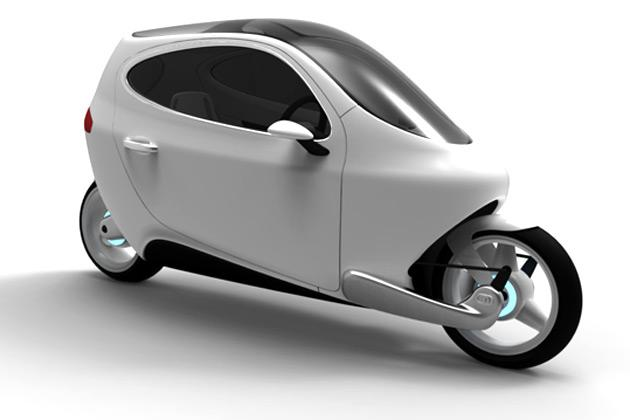
\includegraphics[width=0.4\linewidth]{fig1.png}
		\caption{Two-wheeled self-balancing car}
		\label{fig1}
	\end{figure} 
	
	The two-wheeled vehicle is composed of a cart system, a steering system (front part) and a body (rear part). Driven by the DC servo motor, the cart and steering systems allow drivers to change cart position and handle angle. To simplify the modeling in this mini-project, the self-balance two-wheeled vehicle is assumed to be stationary and the mechanical structure is given in Fig.~\ref{fig2}.
	
	\begin{figure}[htbp]
		\centering
		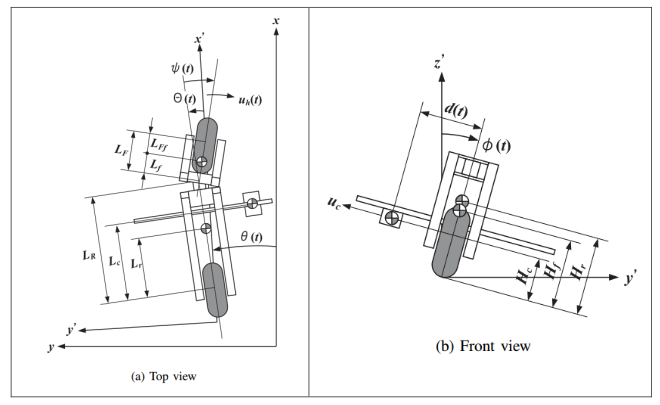
\includegraphics[width=0.6\linewidth]{fig2.png}
		\caption{Simple two-wheeled vehicle model}
		\label{fig2}
	\end{figure} 
	
	Then, state space model is established
	
	\begin{equation}
	\begin{split}
	\begin{aligned}
		\dot{x}&=Ax+Bu \\
		y&=Cx
	\label{eq1}
	\end{aligned}
	\end{split}
	\end{equation}
	
	where the state is designed according to the cart position, handle angle, bike angle and their corresponding velocities respectively
	
	\begin{equation}
		x=\begin{bmatrix}
		d(t) & \phi(t) & \psi(t) & \dot{d}(t) & \dot{\phi}(t) & \dot{\psi}(t) 
		\end{bmatrix}^{T}
	\label{eq2}
	\end{equation}
	
	and the relative matrices and input vectors are
	
	\begin{equation}
		A=\begin{bmatrix}
		0 &0  &0  &1  &0  &0 \\ 
		0 &0  &0  &0  &1  &0 \\ 
		0 &0  &0  &0  &0  &1 \\ 
		0 &6.5  &-10  &-\alpha   &0  &0 \\ 
		a_{51} &a_{52}  &a_{53}  &a_{54}  &a_{55}  &a_{56} \\ 
		5 &-3.6  &0  &0  &0  &-\gamma  
		\end{bmatrix}, 
		B=\begin{bmatrix}
		0 &0 \\ 
		0 &0 \\ 
		0 &0 \\ 
		\beta  &11.2 \\ 
		b_{51} &b_{52} \\ 
		40 &\delta  
		\end{bmatrix}
	\label{eq3}
	\end{equation}
	
	\begin{equation}
		C=\begin{bmatrix}
		1 &0  &0  &0  &0  &0 \\ 
		0 &1  &0  &0  &0  &0 \\ 
		0 &0  &1  &0  &0  &0 
		\end{bmatrix},
		D=\begin{bmatrix}
		u_{c}(t) &u_{h}(t) 
		\end{bmatrix}^{T}
	\label{eq4}
	\end{equation}
	
	The parameters in matrix $A$ and $B$ can be calculated as
	
	\begin{equation}
		%\begin{gather}
	\begin{split}
			a_{51}&=-\frac{M_{c}g}{den},
			a_{52}=\frac{(M_{f}H_{f}+M_{r}H_{r}+M_{c}H_{c})g}{den}, 
			a_{53}=\frac{(M_{r}L_{r}L_{F}+M_{c}L_{c}L_{F}+M_{f}L_{Ff}L_{R})g}{(L_{R}+L_{F})den}\\
			a_{54}&=-\frac{M_{c}H_{c}\alpha}{den},
			a_{55}=-\frac{\mu _{x}}{den},
			a_{56}=\frac{M_{f}H_{f}L_{Ff}\gamma }{den}\\		
			b_{51}&=\frac{M_{c}H_{c}\alpha }{den},
			b_{52}=-\frac{M_{f}H_{f}L_{Ff}\delta }{den},
			den=M_{f}H_{f}^{2}+M_{r}H_{r}^2+M_{c}H_{c}^{2}+J_{x}
			\label{eq5}			
		%\end{gather}
	\end{split}
	\end{equation}
	
	The physical parameters appering in Eq.~\ref{eq4} and Eq.~\ref{eq5} are usually measured mannually by experiments and they are given in appendix.
	
	After obtaining the linear system model and giving a step reference signal for each input channel, two basic response performance specifications are required to meet as follows
	
	\begin{itemize}
		\item The overshoot of system should below 10\%.
		\item The 2\% settling time should be less than 5 seconds.
	\end{itemize}

	The rest of the report is structured in the following manner: In section 2 a state feedback controller is designed using pole placement methods, followed by a discussion on effects of different pole choices. Section 3 concludes a Linear Quadratic Regulator controller design as well as the techique on choosing the weighting matrixes $Q$ and $R$. Section 4 introduces a state observer based on the former LQR control system and its performance is evaluated by monitoring the state estimation error. Section 5 describes a decoupling controller for a 2-input-2-output system. Section 6 designes a controller enabling the output of plant to track the reference signal regardless of step disturbances in input channel. Section 7 tries the integral control method to maintain outputs at a constatnt set point with zero steady-state error. Section 8 concludes the work.
	
	\section{State feedback controller by pole placement method}
	
	\subsection{Method description}
	
	\hspace{1.0em}
	Given the acquired six-order state space model, feedback controller is required to make the system stable. In this section, pole placement method will be used to obtain the feedback gain to meet control requirements. Firstly considering a second-order system, its overshoot and 2\% settling time of a step response is given as follows
	
	\begin{equation}
	M_{p}=e^{\frac{-\pi \zeta }{\sqrt{1-\zeta ^{2}}}}, t_{s}=\frac{4.0}{\zeta \omega _{n}}
	\label{eq6}
	\end{equation}
	
	where $\zeta$ and $\omega_{n}$ are damping ratio and natural frequency respectively. Now that the overshoot should below 10\% and settling time less than 5s, we set $\zeta=0.8$ and $\omega_{n}=1.25$ in this case, and then the two pole of second-order system is calculated as
	
	\begin{equation}
	\lambda _{1,2}=-\zeta \omega _{n}\pm j\omega _{n}\sqrt{1-\zeta ^{2}}
	\label{eq7}
	\end{equation}
	
	To assure the stability of system, the two dominant poles should have little smaller real parts, so we set them at $\lambda_{1,2}=-2.5\pm j1.875$. The other 4 poles are chosen much faster than the two dominant poles. Then the desired characteristic polynomial becomes
	
	\begin{equation}
	\begin{split}
	\begin{aligned}
		\phi _{d}(s)&=(s-\lambda _{1})(s-\lambda _{2})(s-\lambda _{3})(s-\lambda _{4})(s-\lambda _{5})(s-\lambda _{6})\\
		&=s^{6}+a_{5}s^{5}+a_{4}s^{4}+a_{3}s^{3}+a_{2}s^{2}+a_{1}s+a_{0}
	\end{aligned}
	\end{split}
	\label{eq8}
	\end{equation}
	
	The desired closed-loop matrix can be written in controllable canonical form
	
	\begin{equation}
	A_{d}=\begin{bmatrix}
	0 &  1&0  &0  &0  &0 \\ 
	0 &0  &1  &0  &0  &0 \\ 
	0 &0  &0  &1  &0  &0 \\ 
	0 &0  &0  &0  &1  &0 \\ 
	0 &0  &0  &0  &0  &1 \\ 
	-a_{5} &-a_{4}  &-a_{3}  & -a_{2} &-a_{1}  & -a_{0}
	\end{bmatrix}
	\label{eq9}
	\end{equation}
	
	Then the remainning task is transform the system with state feedback also to the controllable canonical form. First compute the controllability matrix and check if it is full rank
	
	\begin{equation}
	W_{c}=\begin{Bmatrix}
	B &AB  &A^{2}B  &A^{3}B &A^{4}B  & A^{5}B
	\end{Bmatrix}
	\label{eq10}
	\end{equation}
	
	Then select 6 independent vectors from $W_{c}$ in the strict order from left to right (the first six column vectors in this case) and group them in matrix X in the following form
	
	\begin{equation}
	X=\begin{Bmatrix}
	b_{1} &b_{2}  &Ab_{1}  &Ab_{2}  &A^{2}b_{1}  &A^{2}b_{2} 
	\end{Bmatrix}
	\label{eq11}
	\end{equation}
	
	Also compute the inverse of $X$ and write it as the following form
	
	\begin{equation}
	X^{-1}=\begin{bmatrix}
	q_{1}^{T} & q_{2}^{T} & q_{3}^{T} & q_{4}^{T} & q_{5}^{T} & q_{6}^{T}
	\end{bmatrix}^{T}
	\label{eq12}
	\end{equation}
	
	Because that the system has multiple input channels, choose the $3^{th} (d_{1}=3)$ and $6^{th} (d_{1}+d_{2}=6)$ row vectors of $X^{-1}$ and construct transformation matrix $T$ as
	
	\begin{equation}
	T=\begin{bmatrix}
	q_{3}^{T} &q_{3}^{T}A  &q_{3}^{T}A^{2}  & q_{6}^{T} &q_{6}^{T}A  &q_{6}^{T}A^{2}
	\end{bmatrix}^{T}
	\label{eq13}
	\end{equation}
	
	Define the feedback gain matrix $\bar{K}\in \mathbb{R}^{2\times 6}$ with 12 unknown variables, we can solve it by establishing the equation
	
	\begin{equation}
	\bar{A}-\bar{B}\bar{K}=A_{d}
	\label{eq14}
	\end{equation}
	
	where $\bar{A}=TAT^{-1}$, $\bar{B}=TB$
	
	After obtainning the matrix $\bar{K}$, we can finally get the original feedback gain matrix $K=\bar{K}T$. Substitute the control law $u=-Kx+r$ into Eq.~\ref{eq1} and the new closed-loop system becomes
	
	\begin{equation}
	\begin{split}
	\begin{aligned}
	\dot{x}&=(A-BK)x+Br \\
	y&=Cx
	\label{eq15}
	\end{aligned}
	\end{split}
	\end{equation}
	
	
	\subsection{Simulation results}
	
	Pole placement
	
	
	Size\cite{b1}
	
	\subsection{Discussion and refinements}
	
	\section{...}
	...
	\section{Conclusion}
	\section*{Acknowledgments}
	%MS++++++++++++++++++++++++++++++ Reference ++++++++++++++++++
	%% 参考文献请看下一节详细介绍。
	
	\bibliographystyle{IEEEtran}
	
	\bibliography{ref_5401}{}
	
\end{document}